\section{Evaluation}
\par In this section, we will evaluate 1) the Agda code based on the
different representations of mathematical objects that we have chosen and 2) the
development process. Furthermore, we will discuss the feasibility of
formalising mathematics and programming logic in practice based on our own experiences. 


\subsection{Different choices of representations}
\par In computer proofs, an abstract mathematical
object usually requires a concrete representation. The consequence is that different representations will lead to different
formalisations and thus contribute to the
easiness or difficulty in completing the proofs. In the
following paragraphs, we will discuss the decisions we have made and
their effects on the project. 

\paragraph{The set of states (Q) and its subsets} As we have mentioned
in section 3, Firsov and Uustalu represent the set of states \mb{Q} and its subsets
as column matrices in their work \cite{firsov2013}. However, this representation looks unnatural compare
to the actual mathematical definition. Therefore, at the beginning, we intended to avoid the vector representation and to
represent the sets in abstract forms. In our approach, the set of states are represented as a data type in Agda, i.e. \mb{Q : Set}, and its
subsets are represented as unary functions on \mb{Q}, i.e. \mb{DecSubset\ Q = Q \to
  Bool}. 

\par Our definition allows us to finish the proofs in
\textbf{Correctness/RegExp-eNFA.agda} without having to
manipulate matrices. The proofs also look much more natural compare to that in
\cite{firsov2013}. However, there is a problem when the sets have to be iterated when computing the 
\(\epsilon\)-closures because this representation is not possible to
iterate. Therefore, in the current version, several extra fields are included in the automata
including \mb{It} -- a vector containing all the states in \mb{Q}. With \mb{It}, the subsets
of \mb{Q} can be iterated by applying their own functions \mb{Q \to
  Bool} to all the elements in \mb{It}. Note that the
vector \mb{It} is equivalent to the vector representation of the set of
states. 

\paragraph{The languages accepted by regular expressions and finite automata} At first, the
accepting language of regular expressions was defined as a decidable
subset, i.e. \mb{L^R : RegExp \to DecSubset\ \Sigma^*}. The decision
was reasonable because the language has been proved decidable for many
years. However, when we were defining the language, we
were also constructing a boolean decider for regular
expressions. The definition added a great amount of
difficulties in writing the proofs because the proofs had to be built
based on the decider. For example, in the concatenation case, an extra recursive
function was needed to iterate different combinations of input
string. Furthermore, the decidability of the language is not
necessary in proving the equality. Therefore, in the current version, the language
is defined as a general subset, i.e. \mb{L^R : RegExp \to Subset\
  \Sigma^*}. This definition allows us to separate out the decider from
the mathematical definition and to prove their equality in an abstract level. 

\par The same situation also applies to the accepting language of finite automata. At first, the
accepting language of NFA was obtained by running an algorithm that
produces all the reachable states from \mb{q_0} using the input
string. The algorithm was also a decider for NFA. Once again, this
definition mixes the decider and the proposition together
and the decidability of NFA is not necessary in the equality. Therefore, in the current
version, the accepting language of NFA is defined in an abstract form. 

\par However, this does not mean that we can ignore the algorithms. In
fact, the decidability of DFA requires an algorithm to return the last
state after running the DFA. In this case, the correctness proof of the
algorithm is required. However, compare to the algorithm used in
running NFA, this algorithm is much simpler which also
makes its correctness proof very easy to finish. Furthermore, the
decidability of NFA and regular
expressions follows directly after their accepting languages are
proved to be equal. 

\paragraph{The set of reachable states from \(q_0\)} Let us recall the
definition of reachable states from \mb{q_0}. 
\begin{center} 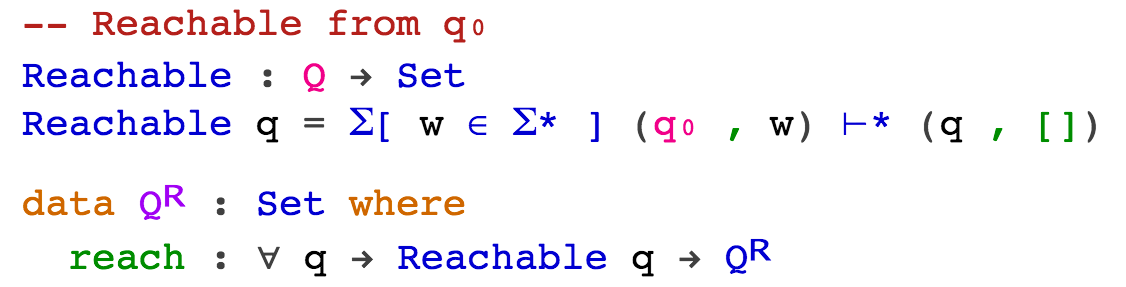
\includegraphics[width=.6\textwidth]{reach} \end{center}

\par We say that a state \mb{q} is reachable if and
only if there exists a string \mb{w} that can take \mb{q_0} to
\mb{q}. Therefore, the set \mb{Q^R} should contains all and only the
reachable states in \mb{Q}. However, there may exist more than one
reachability proof for a single state. This implies that there may be
more than one element in \mb{Q^R} having the same state in \mb{Q}. Therefore, \mb{Q^R}
may be larger than the original set \mb{Q} or even worse, it may be
infinite. This leads to a problem when a DFA is constructed using
\mb{Q^R} as the set of states. If \mb{Q^R} is
infinite, then there is no possible way to iterate the set during 
quotient construction. Even if the set \mb{Q^R} is finite, it
contradicts our original intention to minimise the set of states. This is also one of the
reasons why our formalisation of quotient construction cannot be
completed. However, this has no effects on the proof of \mb{L(DFA) =
  L(MDFA)} because we can provide an equality relation of states of
a DFA. In the translation from DFA to MDFA, we defined
the equality relation as follow: any two states in \mb{Q^R} are equal if and only
if the input states are equal. Therefore, two elements with same state
but different reachability proofs are still considered the same in the new DFA. 

\par One possible way to solve the problem is to re-define the
reachability of a state such that any reachable state will have a
unique reachability proof. For example, the representative proof can
be selected by choosing the shortest string \mb{(w)} sorted according
to alphabetical order. This also requires a proof that
the chosen representative is unique. Another solution is to use
homotopy type to declare the set \mb{Q^R}. This type allows us to
group different reachability proofs into a single element such that
every state will only appear once in \mb{Q^R}. 


\subsection{Development Process}
\par As we have mentioned before, the parts related to quotient
construction were not completed. One of the reasons
has been discussed in the previous part. However, the major reason is
that there was only very limited time left when we started the quotient
construction. In the following paragraphs, we will evaluate the whole
development process and discuss what could have been done better. 

\par In the first 6 weeks, I was struggling to find
the most suitable representations for regular expressions, finite
automata and their accepting languages. During the time, I was
rushing in coding without thinking about the whole picture of
the theory. As a result, many bad decisions had been made, for example, omitting the
\(\epsilon\)-transitions in the translation process and trying to prove
the decidability of regular expressions directly. After taking the
advice from my supervisor, I followed the definitions in the
book \cite{aho1972} and started writing a framework of the
theory. After that, in just one week, the Agda
codes that formed the basis of the final version were developed by
using the framework. One could argue that the work
done in the first 6 weeks also contribute to those Agda codes but
there is no doubt the written framework highly influenced the
development. Therefore, even though it is convenient to write proofs
using the interactive features in Agda,
it would still be better to start with a framework in early stages. 

\par After that, the development went smooth until the first week of
the second semester. During the time, I started to prove several
properties of \(\epsilon\)-closures. The plan was to finish this part
within 2 weeks. However, 4 weeks were spent on it and very little
progress were made. These 4 weeks were crucial to the schedule and
the time should have been spent more wisely on other parts of the
project such as powerset construction and the report. 


\subsection{Computer-aided verification in practice}
\par In order to evaluate the feasibility of performing computer-aided verification in
practice, we will discuss:1) the difference between computer proofs and written proofs, 2) the easiness or
difficulty in formalising mathematics and programming logic and 3) the
difference between computer-aided verification and testing. 


\subsubsection{Computer proofs and written proofs}
\par According to Geuvers \cite{geuvers2009}, a proof has two major roles: 1)
to convince the readers that a statement is correct and 2) to explain
why a statement is correct. The first role requires the proof to be
convincing. The second role requires the proof to be able to give an
intuition of why the statement is correct. 

\paragraph{Correctness} Traditionally, when mathematicians submit
the proof of their concepts, a group of other mathematicians will
evaluate and check the correctness of the proof. Alternatively, if the
proof is formalised in a proof assistant, it will be checked 
automatically by the compiler. The only difference is that we are now
relying on the compiler and the machine that runs the compile rather
than the group of mathematicians. Therefore, if the compiler and the
machine work properly, then any formalised proof that
can be compiled without errors is said to be correct. Furthermore, a
proof can been seen as a group of smaller reasoning steps. We can say that the a proof is correct if and only if all the
reasoning steps within the proof are correct. When writing proofs in paper, the proofs of
some obvious lemmas are usually omitted and this sometimes leads to mistakes. However, in
most proof assistants, the proofs of every lemma must be provided explicitly. Therefore, the correctness of
a computer proof always depends on the correctness of the smaller reasoning steps within it. 

\paragraph{Readability} The second purpose of a proof is to explain why
a certain statement is correct. Let us consider the following code
snippet extracted from \textbf{Correctness/RegExp-eNFA.agda}. 
\begin{center} 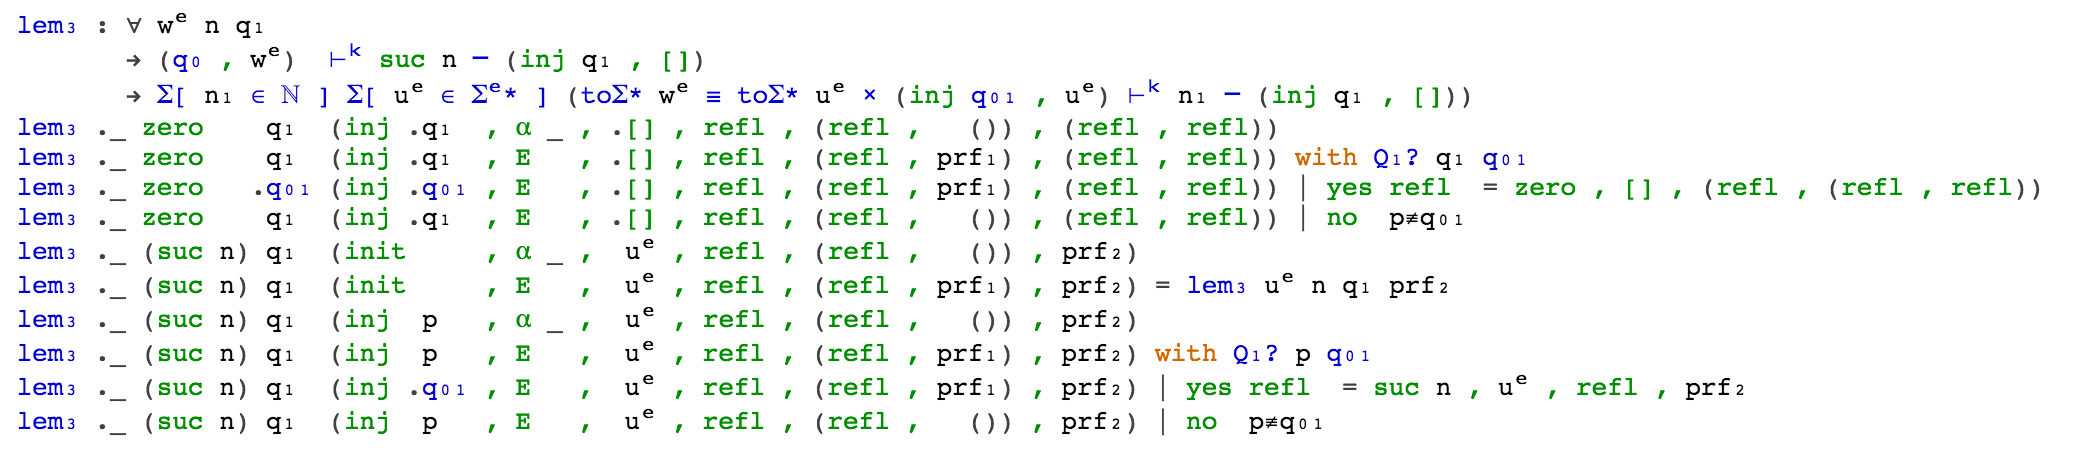
\includegraphics[width=\textwidth]{code} \end{center}

\par The above code is a proof that if \mb{w^e} can take \mb{q_0} to
another state \mb{inj\ q_1} in an \(\epsilon\)-NFA translated from a
regular expression \mb{e^*}, then there exists a number \mb{n_1} and
an \(\epsilon\)-string \mb{u^e} that will take \mb{inj\ q_{01}} to \mb{inj\ q_1} where
\mb{q_{01}} is the start state of \mb{e} and \mb{q_1} is a state in
\mb{e}. There are several techniques used in the proof including the 
induction on natural numbers and case analysis on state comparison. However, by
just looking at the function body, the proving process can hardly be
understood. Therefore, in general, a computer proof is very inadequate on
this purpose and thus an outline of the proof in natural language is
still necessary. 

\paragraph{} Although computer proof seems to be unreadable, the advantages
are still impressive. For example, a group
of mathematicians may need months to validate a very long piece of
proof, but a computer proof may only need days to
compile. 


\subsubsection{Easiness or difficulty in the process of formalisation}
\par As a computer science student without a strong mathematical
background, I find it not very difficult to do the
formalisation as there are many similarities between writing codes and writing
proofs, for examples, pattern matching and case analysis, recursive
function and mathematical induction. Furthermore, Agda is convenient
to use for its interactive features. The features allow us to know
what is happening inside the proof body easily by showing the goal and all the
elements in the proof. Also, many theorems can be automatically proved
by Agda. 
\par On the other hand, most of the
proof assistants based on dependent types support only primitive or
structural recursion. Many algorithms can be very difficult to
implement under this limitation. For example, the usual algorithm that is used to compute
\(\epsilon\)-closure is as follow:
\begin{lstlisting}[mathescape=true,xleftmargin=.3\textwidth]
Suppose we are finding the $\epsilon$-closure of a state $q$:
1) Let $A$ be a set of states
2) Put $q$ in the set $A$
3) Loop until there is no new elements add to $A$
  3.1) For every state $p$ in $A$, if another state $r$ is reachable
       from $p$ with one $\epsilon$-transition, we put it in $A$
4) The resulting set $A$ is the $\epsilon$-closure of $q$
\end{lstlisting} 
\par This kind of algorithms cannot be implemented directly without
modifications. Furthermore, most of the proof assistants are
not Turing-complete which means that there
might be some useful algorithms which cannot be expressed. 


\subsubsection{Computer-aided verification and testing}
\par The most common way to verify a program is via testing. However,
no matter how sophisticated the design of the test cases is, the
program still cannot be proved to be 100\% correct. On the other
hand, total correctness can be achieved by proving the specifications
of a program. Already in 1997, Necula \cite{necula1997} has raised the
notion of \textit{Proof Carrying code}. The idea is to accompany
program with several proofs that proves the program specifications
within within the same platform. In fact, there is already an
extraction mechanism \cite{letouzey2008} in Coq that allows us to
extract proofs and functions in Coq into Ocaml, Haskell or Scheme
programs. 

\par programming logic like concurrency? what about distributive
system? cloud?  ... 